\documentclass[10pt,a4paper]{amsart}
\usepackage[margin=19mm]{geometry}
\usepackage{amsmath,amssymb,mathtools}
\usepackage[scr=rsfs,cal=euler]{mathalfa}
\usepackage{xfrac}
\usepackage[unicode,hidelinks,bookmarks=false]{hyperref}
\newcommand{\ie}{i.e.\ }
\newcommand{\cf}{cf.\ }
\newcommand{\resp}{respectively\ }
\newcommand{\Subsection}{\subsection}
\providecommand{\nobreakdash}{\nobreak\hbox{-}}
\setlength{\emergencystretch}{2em}
\multlinegap0pt
\usepackage{amssymb}
\usepackage{enumerate}
\usepackage{tikz}
\usepackage{bm}
\usepackage{csquotes}
\newtheorem{lemma}{Lemma}
\newcommand{\Dual}{D}
\newcommand{\mysetminus}{\mathbin{\mathchoice{\mysetminusD}{\mysetminusT}{\mysetminusS}{\mysetminusSS}}}%according to the maths size
\newcommand{\mysetminusD}{\hbox{\tikz{\draw[line width=0.6pt,line cap=round] (3pt,0) -- (0,6pt);}}}
\newcommand{\mysetminusS}{\hbox{\tikz{\draw[line width=0.45pt,line cap=round] (2pt,0) -- (0,4pt);}}}
\newcommand{\mysetminusSS}{\hbox{\tikz{\draw[line width=0.4pt,line cap=round] (1.5pt,0) -- (0,3pt);}}}
\newcommand{\mysetminusT}{\mysetminusD}
\newcommand{\oPerpStar}{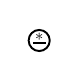
\begin{tikzpicture}[scale=0.134]
\draw[thick,line width=0.7pt](-0.6,-0.2)--(0.6,-0.2) ;
    \draw (0,0.1) node[scale=0.6] {\rm{*}};
  \draw[line width=0.7pt] (0,0) circle [radius=1];
\end{tikzpicture}}
\newcommand{\oPerpstar}{\mathbin{\raisebox{-1pt}{\oPerpStar}}}
\title{One-ended spanning subforests and treeability of groups}
\author{Clinton T. Conley, Damien Gaboriau, Andrew S. Marks, Robin D. Tucker-Drob}
\date{Source: arXiv:2104.07431v3 (CC BY 4.0)}
\begin{document}
\maketitle

\noindent\emph{Source and licence.} One-ended spanning subforests and treeability of groups. Version arXiv:2104.07431v3 (CC BY 4.0), distributed by arXiv under the Creative Commons Attribution 4.0 International licence, http://creativecommons.org/licenses/by/4.0/, as recorded in the arXiv licence metadata for this exact version and shown on the abstract page https://arxiv.org/abs/2104.07431v3. Full licence notice: \texttt{licenses/arxiv-2104.07431-CC-BY-4.0.txt}.\par\smallskip

\noindent\textit{Editorial scope.} Counted unit: the article's lemma lem:back-orbit\_retraction (source0.tex lines 1725--1727). The article's complete original proof of it is delivered with it (source0.tex lines 1729--1747, one \texttt{proof} environment of 19 lines). No mathematics is written, repaired or re-derived: the statement and the proof are the article's own lines, in the article's own notation, and no retained line is substituted or re-flowed.  No further source-local context is needed: every cross-reference of every retained line resolves inside the two delivered spans.  Nothing was omitted from any retained span, so the package carries no omission record.  No retained line contains a citation, so the wrapper carries no bibliography and no bibliography entry.  No retained line contains a figure environment, an image-inclusion command or drawing code, so no image is delivered and the package declares no asset dependency.  Editorial formatting only, in addition: an AMS \texttt{amsart} preamble that restates the article's own declarations and macros used by the retained lines, namely the environments \texttt{lemma} on separate counters, together with the standard packages those lines need.  The retained environments print in this document as Lemma 1 in order of appearance, whereas the article prints the same items with the numbering of its own full document.  The complete native source of the article as distributed in the arXiv e-print for this exact version is bundled unchanged as \texttt{sources/110351/source0.tex}.
\begin{lemma}\label{lem:back-orbit_retraction}
If $L$ is a compact ${\mathtt{F}^{*}}$-back-orbit saturated subcomplex of ${\Sigma} $, then it admits a retraction to $L\cap ({\Sigma}\oPerpstar {{\mathtt{F}^{*}}})$.
\end{lemma}

\begin{proof}
The key point is that any simplex admits a retraction to its boundary minus any one of its faces.
We then argue by a decreasing induction on the number of $d$-dimensional cells of $L$:
\\
Observe if $L$ has no $d$-dimensional cells then it has to be contained in ${\Sigma}\oPerpstar {{\mathtt{F}^{*}}}$.
\\
Otherwise, pick $\epsilon$ one of the $n\geq 1$ cells of dimension $d$ of $L$.
Consider in ${\mathtt{F}^{*}}$ the unique path $p$ from $\Dual_{d}^{-1}(\epsilon)$ to the infinite end.
By finiteness of $L$ there is a least vertex $v\in p\cap \Dual_{d}^{-1}(L)$.
By definition $\sigma:=\Dual_{d}(v)$ and $\tau:=\Dual_{d-1}(o(v))$ are cells of $L$.



Claim:
Removing $\sigma$ and $\tau$ from $L$ delivers a ${\mathtt{F}^{*}}$-back-orbit saturated subcomplex $L_{\sigma}\subseteq L$ of ${\Sigma} $ with one $d$-dimensional cell less, together with a retraction $U_{\sigma}: L\to L_{\sigma}$. 
This is because, by construction, the cell $\sigma$ doesn't belong to the back-orbit of any other $(d-1)$-dimensional cell of $L$ than $\tau$.
The cell $\sigma$ admits a retraction $V_{\sigma}$ to $(\partial \sigma)\mysetminus \tau$ (its boundary minus $\tau$), which extends (by the identity) on the rest of $L$.

Now, a decreasing induction gives successive retractions $U_{\sigma_1}, U_{\sigma_2}, \cdots, U_{\sigma_n}$ whose composition is a retraction from $L$ to a subcomplex contained in ${\Sigma}\oPerpstar {{\mathtt{F}^{*}}}$. This completes the proof of the lemma.\end{proof}

\end{document}
